\documentclass[unnumsec,webpdf,contemporary,large]{oup-authoring-template}
%% OUP authoring template (v1.5), bundled in this package so that it compiles
%% on Overleaf without requiring the class to be installed separately.

\usepackage[T1]{fontenc}
\usepackage{lmodern}
\usepackage{booktabs}
\usepackage{graphicx}
\usepackage{amsmath}
\usepackage{amssymb}
\usepackage{textcomp}
\usepackage{xurl}
\usepackage{microtype}
\usepackage[hidelinks]{hyperref}

%% The class expects a society logo hook; empty means no logo.
\def\societylogo{}

% Local fix for the bundled class's opening header: the 4 mm left ornament
% must be subtracted from the nested header box, not added beyond textwidth.
% Body dimensions and the supplied class file remain unchanged.
\usepackage{etoolbox}
\makeatletter
\patchcmd{\ps@opening}{\vskip2.5pt\hbox to \textwidth}{\vskip2.5pt\hbox to \dimexpr\textwidth-4mm\relax}{}{\PackageError{bib-revision}{Opening odd header patch failed}{Inspect the bundled class.}}
\patchcmd{\ps@opening}{\vskip2.5pt\hbox to \textwidth}{\vskip2.5pt\hbox to \dimexpr\textwidth-4mm\relax}{}{\PackageError{bib-revision}{Opening even header patch failed}{Inspect the bundled class.}}
% Manuscript page headers; production metadata is assigned by the publisher.
\def\ps@opening{\def\@oddhead{\small\itshape Briefings in Bioinformatics\hfill Problem solving protocol}\let\@evenhead\@oddhead\def\@oddfoot{\hfil\thepage\hfil}\let\@evenfoot\@oddfoot}
\def\ps@manuscript{\def\@oddhead{\small\itshape Reconstruction and generation in AMP design\hfill\thepage}\let\@evenhead\@oddhead\let\@oddfoot\@empty\let\@evenfoot\@empty}
\makeatother

\graphicspath{{figures/}}

\begin{document}

\journaltitle{Briefings in Bioinformatics}
\DOI{}
\copyrightyear{2026}
\pubyear{2026}
\vol{}
\issue{}
\access{}
\appnotes{Problem solving protocol}
\firstpage{1}

\title[Reconstruction and generation in AMP design]{Reconstruction gains in antimicrobial peptide generation do not establish generative superiority}

\author[1,2,$\ast$]{Hongsheng Wang\ORCID{0009-0009-8214-5150}}
\author[1]{Fei Wu\ORCID{0000-0003-2139-8807}}
\author[3]{Feng Lin\ORCID{0000-0002-1199-5870}}

\address[1]{\orgdiv{College of Computer Science and Technology}, \orgname{Zhejiang University}, \orgaddress{\street{866 Yuhangtang Road, Xihu District}, \postcode{310058}, \state{Zhejiang}, \country{China}}}
\address[2]{\orgdiv{Artificial Intelligence Department}, \orgname{Loctek Ergonomic Technology Corp.}, \orgaddress{\street{Loctek Building, 436 Xueshi Road, Shounan Subdistrict, Yinzhou District}, \postcode{315100}, \state{Zhejiang}, \country{China}}}
\address[3]{\orgname{Fuyao University of Science and Technology}, \orgaddress{\street{No. 104 Zhihui Avenue, Fuzhou High-tech Industrial Development Zone}, \postcode{350109}, \state{Fujian}, \country{China}}}
\corresp[$\ast$]{Correspondence: Hongsheng Wang. \href{mailto:wanghongsheng@zju.edu.cn}{wanghongsheng@zju.edu.cn}}

\abstract{Reconstruction, sequence-distribution similarity and antibacterial activity are distinct endpoints in antimicrobial peptide generation. We evaluate a reconstruction-objective change within one fixed development protocol. With matched architecture, initialization, batches, decoder and training schedule, a 21-class categorical objective (CE21) raises development residue micro accuracy from 12.55\% to 70.90\% relative to squared error (MSE21). CE21 improves six specified sequence-distribution distances in both terminal conditions and against both references, but a terminal-conditioned LSTM remains closer on all 24 comparisons. These descriptive results use one training seed and a development set used during model development; fixed KL weighting does not hold effective regularization constant. Seven exploratory routes give diagnostic and gate outcomes that do not establish improved generation. A separate historical laboratory case study includes 30 ordered and 27 assayed peptides. Retrospective MIC aggregation agrees with 105 of 108 reported summary cells. At a strict \textit{S. aureus} threshold below 200 \textmu{}g/mL, the reported summary gives six active peptides and the retrospective algorithm gives seven; both ordered and assayed denominators are reported. These peptides are not linked to the evaluated models. Comparison with AMPGen illustrates why activity fractions require explicit candidate selection, strain criteria, thresholds, units and denominators. The disclosure framework connects computational endpoints and sample-level laboratory evidence. Reconstruction improvement alone does not establish generative superiority; that claim requires direct generation evaluation and traceable linkage to laboratory evidence.}

\keywords{antimicrobial peptides, generative models, benchmarking, variational autoencoder, diffusion models, reproducibility}

\otherabstract[Author description]{The authors study machine learning for antimicrobial peptide discovery across computer science, industrial artificial intelligence and biotechnology, emphasizing reproducible evaluation and traceable connections between computational design and laboratory measurements.}


\maketitle
\pagestyle{manuscript}
% Keep natural section spacing instead of stretching sparse columns.
\raggedbottom

\section{Introduction}

Many antimicrobial peptides are short cationic sequences studied as templates for antibacterial candidates \cite{ref50,ref51}. Variational autoencoders, adversarial networks and diffusion models propose novel peptides \cite{ref1,ref2,ref3,ref14,ref15,ref16,ref17,ref18,ref19,ref20,ref21}. Candidate discovery also includes virtual-library enumeration, proteome mining and machine-learning-guided design with laboratory assessment \cite{ref22,ref23,ref24}. Evaluation practices nevertheless differ in what constitutes evidence of a generative improvement \cite{ref25}.

Three endpoints are routinely reported, and they are not interchangeable. \textbf{Reconstruction} measures whether a model can reproduce a known sequence from its latent representation, given the sequence itself as input. \textbf{Distributional similarity} measures whether a sampled set resembles a reference set in low-order statistics such as residue and dipeptide composition; metrics of this kind are standard in molecular and sequence generation \cite{ref26,ref27,ref28,ref29}. \textbf{Downstream activity} measures whether synthesized material inhibits a target organism. A model can improve the first without improving the second, and can match residue frequencies while producing no useful activity spectrum.

AMP classifiers and activity predictors illustrate the importance of controlled comparison \cite{ref30,ref31,ref32,ref33,ref34,ref35,ref36,ref37}. Deep models need not outperform shallow models \cite{ref4}; negative-data selection can bias prediction benchmarks \cite{ref5}, while homology-aware partitioning addresses sequence leakage \cite{ref38,ref39}. Related benchmarks \cite{ref6} and reporting standards \cite{ref40,ref41,ref42,ref43,ref44,ref45,ref46} motivate explicit control of data exposure and evaluation conditions.

Published AMP pipelines differ in data, terminal-state handling, sampling, selection and assays \cite{ref1,ref2,ref3,ref7}. Recent work covers AI-driven screening \cite{ref7}, generative-model comparisons \cite{ref8}, diffusion design with assays \cite{ref9}, text-guided generation \cite{ref11}, and quantitative MIC and haemolysis benchmarks \cite{ref13}. We ask whether changing reconstruction loss within one implementation improves reconstruction and sampled-sequence statistics, and whether it exceeds a separately trained comparator.

Training and sampling also differ in variational autoencoders \cite{ref47}, diffusion models \cite{ref48,ref49}, protein representation and structure prediction \cite{ref52,ref53}, and protein design \cite{ref54,ref55,ref56,ref57,ref58,ref59}. A training-objective gain requires direct evaluation of the intended sampled-output endpoint.

We compare CE21 and MSE21 under matched architecture, initialization, batches, decoder and training schedule, changing the reconstruction loss applied to the shared output head. We measure both reconstruction and generation endpoints. This isolates the objective change within the fixed protocol, although it does not hold the effective balance between reconstruction and KL regularization constant. A separately trained, terminal-conditioned LSTM provides an executable comparator for generation.

Our contribution is a bounded evaluation of one development protocol. CE21 improves reconstruction and all six specified distributional distances relative to MSE21, but remains behind the LSTM on the 24 metric--terminal--reference comparisons. A separate laboratory record illustrates why assay outcomes alone cannot establish which evaluated model generated an assayed peptide. We use these two records to distinguish measured endpoints from the evidence needed to connect them.


\section{Materials and methods}

\subsection{Study data and analysis scope}

The computational study uses the AMP implementation derived from \url{https://github.com/3DHumanRehab/AMP} (commit \texttt{e7486fb}) and the fixed experimental wrappers and outputs in \url{https://github.com/wanghongsheng01/amp-claude-handoff-20261013} (commit \texttt{f1b748d}). Supplementary Methods identify the exact source files and configurations. Analyses use the training and development partitions; the reserved evaluation partition was not accessed.

The accompanying materials contain saved reconstruction and generation outputs, activity predictions, assay readouts and a sample manifest. Independent calculations reproduce the reported computational summaries and compare the original MIC summary with a retrospective algorithm. This recalculation does not repeat model training or laboratory experiments. The historical assay samples have no established checkpoint-to-sample linkage to the evaluated models, and prospective timing of the historical selection and endpoint rules is not established.

\subsection{Cohort construction and terminal conditions}

The cohort derives from a fixed, bounded collection of 512 DBAASP detail cards \cite{ref10}; several other curated AMP repositories exist and differ in admission rules \cite{ref60,ref61,ref62,ref63}. Eligibility required an unchanged canonical 1--48-residue monomer sequence, an unmodified N terminus, a free or amidated C terminus, compatible provider molecular graphs, and traceable bacterial MIC metadata. Sequence grouping used global Needleman--Wunsch identity of at least 70\%, counting all alignment columns including gaps, with transitive connected components. Components appearing in the training material were assigned to training or excluded under a fixed exposure rule; all others received a seeded hash assignment with nominal 80/10/10 proportions. Descriptor scaling was fitted on training data only.

The main experiment used a fixed 279-sequence training partition and a 41-sequence development partition, containing 701 non-padding development residues. Free and amidated terminal groups contained 126 and 153 training sequences and 18 and 23 development sequences respectively. Free and amidated sequences are not matched versions of the same sequence, so terminal-group comparisons do not estimate a chemical-modification effect. Terminal state is the only externally supplied condition during generation; no true sequence, residue-aligned descriptor or true length is supplied to any generator. Sequence-derived descriptors remain available to the encoder during reconstruction and training, so reconstruction receives substantially more input information than de novo generation.

The development partition was used during model development and is therefore not an independent confirmation sample. Dataset and code hashes, configurations and execution rules were fixed before the corresponding runs, which does not remove that use.

\subsection{Reconstruction objectives and decoding}

The categorical (CE21) and squared-error (MSE21) models share the same VAE architecture, initialization, batches, random-number schedule, 48-position output, 21-category head and decoding rule. Output categories are the 20 canonical amino acids plus padding. Each VAE has 1,681,549 parameters, including 357 output-head parameters; its diffusion model has 18,612,994 parameters, for 20,294,543 in the two-stage pipeline. A third pipeline replaces the residue-number regression head with a scalar objective and a different normalization, and is reported as a whole-pipeline comparator rather than a single-component ablation.

The two reconstruction objectives differ only in the loss applied to the shared head. Let \texttt{s\_ijc} be the raw score for category \texttt{c} at position \texttt{j} in sample \texttt{i}, \texttt{y\_ij} the target including padding, and \texttt{B} the batch size:

\begin{equation*}
\mathcal{L}_{\mathrm{CE}} = -\frac{1}{48B}\sum_{i}\sum_{j}\log \operatorname{softmax}(s_{ij})_{y_{ij}}
\end{equation*}

\begin{equation*}
\mathcal{L}_{\mathrm{MSE}} = \frac{1}{96B}\sum_{i}\sum_{j}\bigl\lVert s_{ij} - e_{y_{ij}} \bigr\rVert^{2}
\end{equation*}

where \texttt{e\_y} is the one-hot target. MSE is applied to raw scores, with a factor of one half, and both objectives include padding positions. Both are optimized with the same optimizer, learning rate and update count, so the comparison is component-isolated with respect to the output loss.

Generation from the VAE family follows the fixed sampling path: the diffusion model is trained on the posterior parameters, and a latent is drawn and decoded. A fixed KL coefficient does not control effective regularization strength when the reconstruction loss changes, a limitation we return to in the Discussion.

\subsection{Autoregressive comparator}

The comparator has two LSTM layers (hidden width 64), token embeddings of width 32, terminal embeddings of width 8 and 62,501 parameters. Teacher-forced token training and generation from the terminal condition and sampled prefix use an explicit end-of-sequence token and a 48-residue cap. This locally trained recurrent comparator \cite{ref1} uses the same data and generation metrics; it does not reproduce a published system's performance.

\subsection{Training and sampling budgets}

Each VAE received 1,000 updates followed by 1,000 matching diffusion updates; the LSTM received 1,000 updates. Each arm used one configuration and one training seed, with no development-selected checkpoint or hyperparameter search within this comparison. Initialization and VAE/LSTM seeds were 222, the diffusion seed 322, and generation seeds 422 and 423 for the free and amidated conditions. VAE and diffusion batch sizes were 32 and 8. Execution was serial on one CPU thread, with common training and generation ceilings of 2,940 s and 1,800 s.

Equal ceilings and update counts do not equalize realized computation, capacity or optimization quality. The smaller LSTM used less computation. Its development negative log-likelihood increased from 2.6153 at update 200 to 3.1698 at update 1000; only the final checkpoint was used.

The CE21 generation step was interrupted after training and completed from the final checkpoint with zero additional training updates. All four methods produced 32 requests each (16 per terminal condition), giving 128 main-comparison outputs; the continuation is not an independent training replicate.


\subsection{Metrics and interpretation}

Reconstruction uses the posterior mean and compares the rendered sequence to each target position; missing predicted positions count as incorrect. Micro accuracy uses all 701 development residues, and amino-acid macro accuracy averages recall over target-supported residue classes. Whole-sequence exact matches and length mean absolute error are also reported, each with 41 sequences as denominator.

We report execution, canonical-alphabet compliance, length eligibility, uniqueness and exact training-copy counts for all requests. Distribution comparison uses canonical sequences of length 1--48, retaining outputs shorter than five residues and those at the cap; a separate length 5--48 eligibility count is reported and does not retroactively filter the main comparison.

Six distances compare each generated terminal group with the corresponding training and development groups: residue and dipeptide Jensen--Shannon divergence in bits, their L$_1$ distances, length Kolmogorov--Smirnov distance, and biased linear-kernel MMD$^2$. The latter is the squared distance between mean 421-dimensional features: length/48, 20 residue fractions and 400 dipeptide fractions, with each block weighted by $1/\sqrt{3}$. A one-residue sequence has a zero dipeptide block. JS, L$_1$ and entropy use pooled counts; MMD averages per-sequence features. Entropy and exact training-copy counts are complementary diagnostics (Supplementary Methods; Tables S1--S2).

All comparisons are descriptive. No generated sequence is treated as an independent training replicate. We report no significance tests or confidence intervals from a single fitted seed, and do not infer antibacterial activity from sequence statistics or treat a nearest training sequence as generation ground truth.

\subsection{Historical laboratory case study and retrospective MIC analysis}

Thirty peptides were ordered and 27 delivered and assayed against \textit{E. coli} ATCC 25922, \textit{P. aeruginosa} ATCC 27853, \textit{S. aureus} ATCC 29213 and \textit{E. faecalis} ATCC 29212. The original 27 $\times$ 4 MIC summary is retained unchanged. The assay uses ten two-fold dilutions from 1000 to 1.953125 \textmu{}g/mL and three replicate wells per concentration, peptide and strain, with ampicillin, polymyxin B and daptomycin as reference antibiotics. These yield 324 replicate dilution series and 3,240 peptide OD$_{600}$ readings. Susceptibility-testing methods and AMP standardization issues \cite{ref64,ref65,ref66,ref67} motivate explicit reporting of the actual readout and aggregation rule.

For the retrospective algorithm, each replicate endpoint is the lowest tested concentration with OD$_{600}<0.10$; no qualifying concentration is coded as no endpoint. At least two of three identical numeric calls give a numeric cell endpoint. A majority with no endpoint and a lack of consensus are stored separately; both map to the historical N code only when computing agreement with the original summary. This rule describes retrospective consistency and does not establish the rule used before measurement (Table S5).

\section{Results}

\subsection{Categorical reconstruction substantially improves the reconstruction endpoint}

CE21 reconstructs 497 of 701 development residues (70.90\%), compared with 88 (12.55\%) for MSE21 and 111 (15.83\%) for the scalar pipeline (\textbf{Table 1}). The CE21--MSE21 difference is 58.35 percentage points under matched capacity, initialization, schedule and decoder. CE21 returns the correct length for all 41 sequences and reproduces three complete sequences.

\begin{table*}[t]
\caption{Development reconstruction from the posterior mean. Counts and errors use 701 target residues or 41 sequences. The autoregressive model has no corresponding reconstruction task.}
\label{tab:reconstruction}
\centering
\begin{tabular}{lrrrrr}
\toprule
Model & Correct & Micro (\%) & Macro (\%) & Length MAE & Exact \\
\midrule
CE21 & 497/701 & 70.90 & 42.76 & 0.000 & 3/41 \\
MSE21 & 88/701 & 12.55 & 3.57 & 5.561 & 0/41 \\
Scalar & 111/701 & 15.83 & 8.05 & 1.341 & 0/41 \\
\bottomrule
\end{tabular}
\end{table*}

CE21 macro recall is 42.76\%, below its micro accuracy. Eight target-supported classes have zero recall: C, D, E, H, M, N, Q and Y. Improved micro accuracy therefore does not establish balanced residue coverage.

\subsection{CE21 improves distributional distances but remains behind the recurrent comparator}

All eight method--terminal groups produced 16 canonical outputs of length 1--48, unique within each group, with no exact copy of any training sequence. Stricter length 5--48 counts were 14 and 15 for CE21, 16 and 10 for MSE21, and 16 and 16 for both scalar and LSTM, in free and amidated conditions respectively. These describe a finite sample; they do not exclude memorization or imply biological suitability.

CE21 has lower values than MSE21 and scalar on all six sequence-distribution distances, in both terminal conditions and against both references --- a consistent component-level improvement. The LSTM, however, has lower values than CE21 on each of those same 24 comparisons (\textbf{Figure 1}). Development MMD is 0.017328 for CE21 versus 0.011567 for the LSTM in the free condition, and 0.007710 versus 0.007362 in the amidated condition. The amidated difference is small and receives no significance interpretation.

\begin{figure*}[t]
\centering
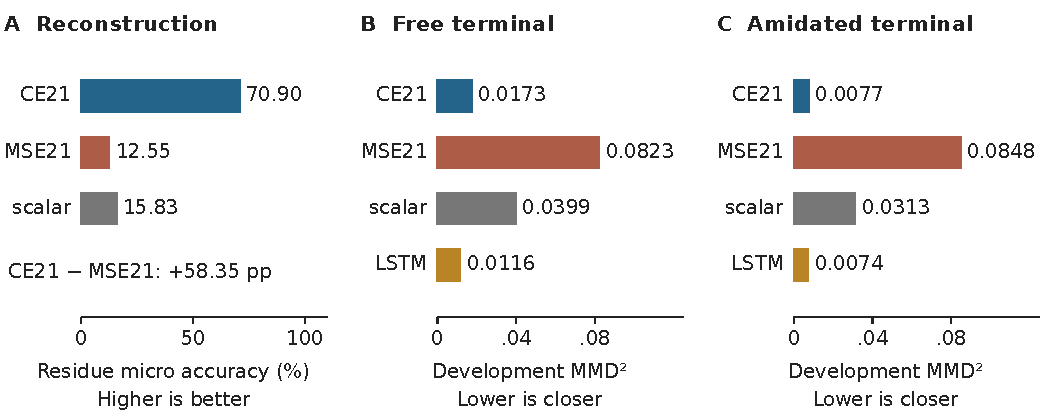
\includegraphics[width=\textwidth]{figures/fig1_reconstruction_vs_generation.pdf}
\caption{Reconstruction and generation under the fixed development protocol. \textbf{(A)} Development residue micro accuracy for the three reconstruction paths. \textbf{(B, C)} Development fixed-feature MMD$^{2}$ for the four generators in free and amidated terminal conditions; lower values indicate closer feature means. CE21 improves on MSE21, while the LSTM is closest on this generation metric. The scalar pipeline is not a matched single-component control. Results use one fitted seed, 701 reconstruction residues and 16 generation requests per method--terminal group; no uncertainty interval is inferred. Values are recalculated from the saved sequences (Tables S1--S2).}\par\smallskip{\small\textbf{Alt text:} Three panels compare reconstruction accuracy and development MMD squared. CE21 reaches 70.90\% reconstruction accuracy versus 12.55\% for MSE21. LSTM has the lowest generation MMD squared in both terminal conditions.}
\end{figure*}


The ordering is not uniform across all diagnostics. Scalar outputs have smaller absolute training-entropy discrepancies than CE21 for both residue and dipeptide entropy under both terminal conditions, and CE21 has fewer length-eligible outputs than scalar or the LSTM, so neither "all generation metrics improve" nor "all distributions worsen" accurately describes the evidence. The descriptive screen applied to the regenerated samples passed all four of its checks; the generation screen failed eight of 18 checks. Those are decision-rule checks, not eight failed sequences, and they do not alter the status of the interrupted generation step reported in Materials and methods.

\subsection{Seven follow-up routes have distinct diagnostic and gate outcomes}

Seven additional diagnostics were run on the same development partition. They investigate the same already-exposed data and are not independent replications.

Training-posterior substitution did not improve development MMD; independent coordinate permutation worsened it. The reference-template prior gave mixed results but used extra template information. These three source diagnostics have no applicable generation winner gate. KL warmup reduced the posterior-mean and eight-draw reconstruction measures from 0.722796 to 0.657852 and 0.661116 to 0.589099, respectively; all four reconstruction/resource guards failed, although its separate investment criterion passed.
Latent-conditioned autoregression passed its information gate (eight-draw score 0.690802 with matched latents, 0.097533 with mismatched latents and 0.091958 for a control trained with permuted latent--sequence pairing) but failed the generation gate. Direct-latent diffusion failed its mechanism screen on MMD and dipeptide JS; its value gate was not interpreted. Safe checkpoint loading rejected an unsupported serialized object, leaving that loading check incomplete; this is not evidence of checkpoint corruption. Saved-sequence metric checks passed.
Conditioning-context variants were not supported by the multistage screen. Equal-terminal development sequence negative log-likelihoods were 49.16431 (partial), 48.58710 (pooled), 48.91772 (separate) and 48.04302 (fresh autoregressive comparator); 384 attempts produced 381 nonempty and three empty outputs. The historical autoregressive value 57.96692 used a different protocol. Full outcomes and definitions are in Table S4. None of these exploratory results establishes improved generation under the tested protocol (\textbf{Figure 2}).


\begin{figure*}[t]
\centering
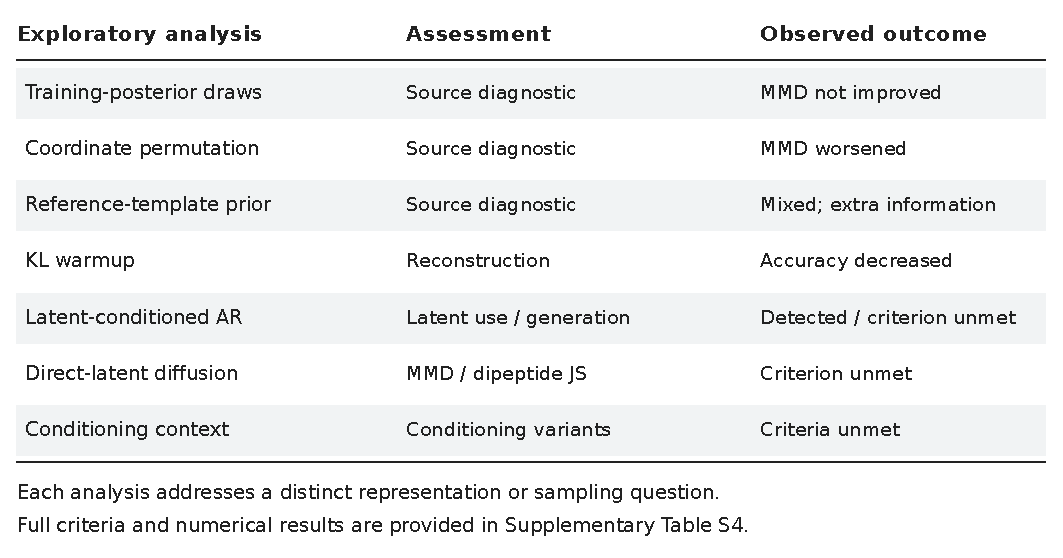
\includegraphics[width=\textwidth]{figures/fig2_route_gates.pdf}
\caption{Distinct outcomes of seven exploratory routes on the development data. The first three are source diagnostics without an applicable generation winner gate. KL warmup fails four reconstruction/resource guards, while its investment criterion passes. Latent-conditioned autoregression passes the information gate and fails the generation gate. Direct-latent diffusion fails the mechanism gate, leaving its value gate uninterpreted. Conditioning-context variants are not supported by their multistage screen. These are configuration-specific outcomes, not independent replications or model-family verdicts (Table S4).}\par\smallskip{\small\textbf{Alt text:} Seven rows list source diagnostics and route-specific outcomes. No common generation gate is assigned to every route. Only latent-conditioned autoregression has an information-pass and generation-fail pair.}
\end{figure*}

\subsection{Exploratory activity modelling did not establish a screening model}

Two activity-modelling experiments on distinct DBAASP development caches \cite{ref10} did not establish a screening predictor (Table S3). Native-unit source-group cross-prediction used 46 mass-unit rows in 10 groups and 39 molar-unit rows in seven groups, with 17 folds and 1,700 convolutional updates. Primary MAE for mean, ridge and CNN predictors was 0.811036, 0.775373 and 0.819758 (mass) and 0.516993, 0.582247 and 0.576262 (molar). The convolutional model, motivated by Witten and colleagues \cite{ref12}, did not beat the mean; the mass-unit ridge advantage reversed under alternative weighting.
The right-censoring comparison used 173 observations (147 point-valued, 26 right-censored), 34 folds, 102 fits and 588 point-validation predictions. Tail-minus-endpoint primary MAE differences were +0.023094 (mass) and +0.137381 (molar). Between-group mean variance accounted for 90.8\% and 71.4\% in the mass and molar groups of this censored-cache diagnostic. Neither activity model selected or validated generated peptides.

\subsection{Parallel reported and retrospective MIC estimates}

The historical case study contains 30 numeric and 78 N cells in the original 108-cell MIC summary; 16 peptides are all-N. The original summary and retrospective algorithm agree in 105/108 cells (97.2\%). Table S5 preserves both representations alongside the underlying OD$_{600}$ readouts.

Three endpoints differ: pp1-1/\textit{S. aureus}, 250 versus 125 \textmu{}g/mL; pp3-14/\textit{P. aeruginosa}, N versus 15.625 \textmu{}g/mL; and pp1-1/\textit{E. faecalis}, 125 \textmu{}g/mL versus no endpoint, for reported versus algorithm estimates. These identified differences have not been experimentally adjudicated; the algorithm is not a determination of the true MIC.

Among the 78 reported N cells, 73 have no numeric replicate endpoint, three have one, one has two and one has three. The last is pp3-14/\textit{P. aeruginosa}, whose three replicates yield 15.625 \textmu{}g/mL. Across all 108 cells, the algorithm gives 30 numeric endpoints, 77 majority-no-endpoint calls and one no-consensus call. N therefore cannot uniformly establish absence of inhibition.

At a strict \textit{S. aureus} MIC threshold below 200 \textmu{}g/mL, the reported summary gives six active peptides: 6/30 ordered (20\%) or 6/27 assayed (22.2\%). The algorithm gives seven: 7/30 (23.3\%) or 7/27 (25.9\%). Neither retrospectively calculated fraction establishes prior commitment to the endpoint.

At strict thresholds below 32, 64, 128 and 200 \textmu{}g/mL, reported \textit{S. aureus} counts are 6, 6, 6 and 6; algorithm counts are 6, 6, 7 and 7. The original gap from 31.25 to 250 \textmu{}g/mL does not apply to the algorithm, which includes 125 \textmu{}g/mL. Activity against any of the four strains below 200 \textmu{}g/mL gives seven peptides under both representations (\textbf{Figure 3}; Table S5).


The reported summary has 11 numeric \textit{S. aureus} and two numeric \textit{P. aeruginosa} entries; the algorithm gives 11 and three, respectively. Figure 3 compares coverage and the \textit{S. aureus} concentration bins without replacing the original summary.

The historical design record describes a 1,000-candidate screen using charge, AMP-prediction score, instability and training-sequence similarity (Supplementary Methods). Thirty peptides were ordered in groups of 8, 8 and 14, labelled broad-spectrum, Gram-positive-specific and Gram-negative-specific; the corresponding assayed counts were 7, 8 and 12. The unassayed identifiers are pp1-6, pp3-8 and pp3-10; their absence does not establish a synthesis-failure cause.


Under the historical operational spectrum-label rule, agreement is 2/8, 1/8 and 0/14 by ordered group, or 3/30 ordered and 3/27 assayed overall, under both MIC representations. This differs from \textit{S. aureus} activity and does not establish biological specificity beyond the four-strain panel; N is treated only as failure to meet the numeric condition.

\begin{figure*}[t]
\centering
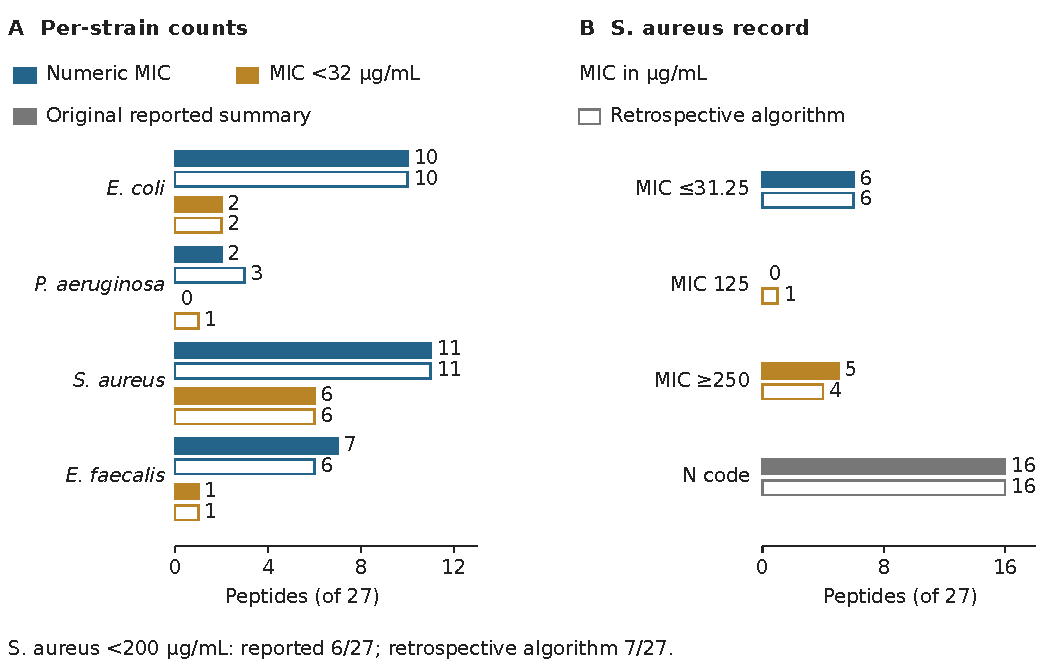
\includegraphics[width=\textwidth]{figures/fig3_mic_checked.pdf}
\caption{Reported and retrospective-algorithm MIC estimates for 27 assayed peptides. \textbf{(A)} Numeric MIC counts and counts strictly below 32 \textmu{}g/mL for each strain, with both representations shown. \textbf{(B)} \textit{S. aureus} distributions: the reported summary contains six values at or below 31.25, five at or above 250 \textmu{}g/mL and 16 N values; the algorithm contains six, four and 16, respectively, plus one value at 125 \textmu{}g/mL. N combines majority-no-endpoint and no-consensus states only for historical comparison. The algorithm does not adjudicate true MIC values.}\par\smallskip{\small\textbf{Alt text:} Filled and outlined bars compare reported and algorithm endpoints by strain. The \textit{S. aureus} distribution changes from five values at or above 250 to four, with one value at 125; its count below 200 changes from six to seven.}
\end{figure*}

Purity certificates show 26 peptides at 95.0--99.1\% and pp1-7 at 80.3\%, meeting its $\geq$80\% order specification. Ten peptides are recorded as insoluble in water and 18 in DPBS; these certificates do not establish the assay solvent. Structural predictions are not experimental structures \cite{ref68,ref69}. Haemolysis and cytotoxicity were not assayed; haemolysis predictors \cite{ref70,ref71,ref72} do not supply such measurements.




\subsection{Comparison with AMPGen under different strain and endpoint definitions}

AMPGen designed 40 peptides and synthesized 38; 31/38 (81.58\%) had MIC $\leq$75 \textmu{}M against \textit{E. coli} K88 or \textit{S. aureus} ATCC 29213 \cite{ref9}. Nine peptides with MIC $<5$ \textmu{}M against both initial targets were subsequently tested against \textit{E. coli} ATCC 25922, \textit{P. aeruginosa} ATCC 27853, \textit{S. aureus} ATCC 25923 and \textit{E. faecalis} ATCC 29212. Thus, the 31/38 fraction does not come from the four-strain extension, and its \textit{S. aureus} extension strain differs from this case study.

The studies use different candidate-selection procedures, strain criteria, thresholds and concentration units. Converting 75 \textmu{}M using the 27 present-case molecular weights gives 80.27625--243.51975 \textmu{}g/mL, illustrating peptide-dependent conversion rather than AMPGen measurement values. Table S6 distinguishes AMPGen's fraction from this case study's reported and algorithm activity fractions and operational spectrum-label agreement.

The differing numerator and denominator definitions are distinct estimands. A harmonized comparison requires peptide-level measurements and common inclusion and activity rules; these data do not assign differences in reported fractions to model performance, biology or criterion choice.


\section{Discussion}

\subsection{Three endpoints, three different claims}

The central empirical finding is that a reconstruction gain of 58.35 percentage points accompanies improved distributional distances over MSE21, but does not exceed the executable LSTM comparator on those distances. The different information available during reconstruction and generation provides a possible explanation, but the present comparisons do not identify the causal mechanism. Reconstruction receives the input sequence and residue-aligned descriptors; sampling receives a terminal condition only.

The latent-conditioned diagnostic shows decodable cached sequence information (0.690802 matched versus 0.097533 mismatched), yet its generation gate fails. It does not isolate optimization, latent-distribution mismatch, decoder behaviour, loss scaling or limited data as the cause. Fixed KL weighting also does not fix effective regularization when reconstruction-loss scaling changes.

\subsection{Interpreting the negative follow-up results}

The seven routes examine latent substitution, prior information, permutation, regularization, decoder conditioning and diffusion targets. Their distinct diagnostics and gates are reported in full, including the incomplete safe-loading check for direct-latent diffusion. These configuration-specific outcomes on exposed development data do not exhaust possible improvements.


\subsection{What the wet-laboratory record establishes}

The historical case study supports endpoint comparison from raw measurements, not attribution of laboratory activity to the evaluated generators. Agreement of 105/108 cells and the parallel six-versus-seven activity counts quantify retrospective consistency. Neither establishes prospective endpoint selection or experimentally adjudicates the three differences.

Raw readings enable retrospective analysis. Linking a physical sample to a generator additionally requires peptide identifiers tied to a checkpoint, configuration and sampling run; assay activity alone cannot establish that link.


We propose six disclosures for an AMP generative claim invoking laboratory evidence (\textbf{Box 1}). \textbf{Figure 4} maps them to this case study without assigning an aggregate score.

\textbf{Box 1. Minimum disclosure for a laboratory-validated AMP generation claim.}

\begin{enumerate}
\item \textbf{Selection protocol, fixed in advance} --- pool size, scoring function, selection rule, and the exact stage at which each peptide was chosen.
\item \textbf{Checkpoint-to-sample linkage} --- model identifier, checkpoint hash, configuration hash and seed for every assayed peptide.
\item \textbf{Denominator and threshold, fixed in advance} --- the strain set, the activity threshold with units, and whether the rule is strict or inclusive, stated before measurement.
\item \textbf{Replicate semantics} --- technical or biological replication, the aggregation rule, and distinct encodings for no endpoint and no consensus.
\item \textbf{Per-sample raw readouts} --- measured values with units, plus explicit encoding of non-numeric outcomes.
\item \textbf{Independence statement} --- whether the evaluation data were used during model development, and whether the comparator models were tuned with an equivalent budget.
\end{enumerate}

The historical selection rules and the retrospective denominator and threshold definitions are stated, but prospective timing is not established. Sample identifiers, raw OD values and both MIC representations are provided; the three differing endpoints remain unadjudicated. Sample-to-checkpoint attribution is not established. Development-data exposure and comparator budgets are disclosed separately and do not establish independent evaluation or equivalent optimization.

\begin{figure*}[t]
\centering
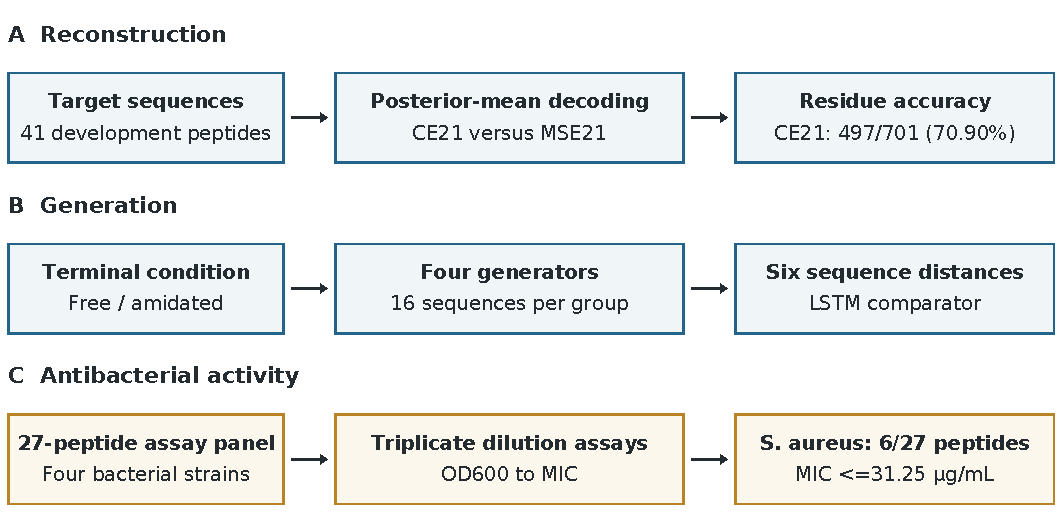
\includegraphics[width=\textwidth]{figures/fig4_evidence_checked.pdf}
\caption{Evidence chain for interpreting the historical laboratory case study. Numbers correspond to Box 1. The historical selection description (1) does not establish decision timing. Sample identifiers and 3,240 raw OD$_{600}$ values (5) support retrospective endpoint comparison (4): 105/108 MIC cells agree and three differ. The reported and algorithm \textit{S. aureus} counts below 200 \textmu{}g/mL are six and seven (3), each using ordered and assayed denominators. These calculations do not adjudicate laboratory MICs. No checkpoint-to-sample assignment is established (2). The computational comparison's data exposure and budgets are disclosed separately (6).}\par\smallskip{\small\textbf{Alt text:} A laboratory evidence chain connects 30 ordered samples, 27 assayed samples and 3,240 optical-density readings to parallel MIC summaries. A missing assignment link separates these samples from model checkpoints. A separate computational panel identifies 279 training and 41 development sequences, one seed and four generators.}
\end{figure*}

\subsection{Relation to prior evaluation work in this journal}

The evaluation follows endpoint-focused AMP-classification critiques \cite{ref4,ref5} and the GPCR--peptide binding benchmark \cite{ref6}, applied here to generation. The matched objective change improves reconstruction and distributional distances over its control but remains behind a separate comparator.

The AMPGen comparison illustrates why overlapping strain identities across different experimental stages do not harmonize success fractions. A generative-superiority claim requires direct generation evaluation, an executable comparator and explicit tuning and data-exposure conditions.

\subsection{Limitations}

The comparison uses one training seed, 16 requests per terminal group and a repeatedly accessed development set, not independent validation. Final-checkpoint LSTM optimization is not established as adequate; further tuning could change the ranking in either direction. Capacity and realized computation differ, and the VAE pipelines additionally train diffusion models. Completing interrupted CE21 generation does not add a replicate.

Activity-modelling caches are small, heterogeneous and exposed. The historical assays have no established attribution to an evaluated model, three unadjudicated endpoint differences, and unverified prospective timing of selection and endpoint rules. The study does not establish biological safety, a general ranking of model families or unsuitability of a model class for peptide design.


\section{Conclusion}

In the fixed 279-training/41-development-sequence protocol, CE21 improves reconstruction from 12.55\% to 70.90\% and all six specified distances over MSE21, while LSTM remains closer on all 24 generation comparisons. These findings concern one seed and exposed development data. The seven exploratory routes do not establish improved generation under their respective diagnostics and gates.

The separate historical case study gives six reported and seven algorithm-derived \textit{S. aureus}-active peptides at the stated threshold. The disclosure framework distinguishes reconstruction, sampled-distribution similarity and laboratory activity, and the sample-level provenance needed to connect those endpoints.

\section*{Funding}

This work was supported by Zhejiang University. No other funding supported this work.

\section*{Author contributions}

\textbf{Hongsheng Wang:} Conceptualization, Methodology, Software, Validation, Formal analysis, Investigation, Data Curation, Writing -- Original Draft, Visualization.

\textbf{Fei Wu:} Conceptualization (academic supervision), Writing -- Review \& Editing, Supervision, Project administration, Funding acquisition.

\textbf{Feng Lin:} Resources; Conceptualization (industrial scenario and requirements); Writing -- Review \& Editing; Supervision (industrial supervisor).

Fei Wu is the guarantor of the work.

\section*{Competing interests}

Hongsheng Wang's affiliation with Loctek Ergonomic Technology Corp. and the institutional collaborations are disclosed in the author list. The authors report no competing interests beyond these disclosed collaborations.

\section*{Relationship to prior work}

Hongsheng Wang and Feng Lin are also authors of AMPGen \cite{ref9}. AMPGen reports a generator with laboratory evaluation; the present study evaluates a reconstruction-objective change and uses a separate historical assay case study. Shared reference-antibiotic and strain identities do not establish comparable study endpoints.

\section*{Ethics statement}

No human participants, human tissue or animal subjects were involved in this work. All bacterial work used the standard reference strains described in Materials and methods.

\section*{Data and code availability}

Saved reconstruction and generation sequences, activity predictions, frozen configurations, analysis code, raw OD$_{600}$ readings, original and retrospective MIC estimates, and sample and purity manifests accompany this manuscript as reviewer materials. Supplementary Tables S1--S6 report the corresponding summaries. Public versioned materials: \url{https://github.com/wanghongsheng01/bib-amp-review-materials-20261023/tree/v3.1-2026-10-23}; materials DOI: \url{https://doi.org/10.5281/zenodo.23586233}. The accompanying offline scripts recalculate summary results without model training or access to the reserved evaluation partition. Source repositories and versions are identified in Materials and methods.

\section*{Acknowledgements and use of generative AI tools}

The authors wrote the manuscript. OpenAI Codex assisted with source and reference checking, code inspection, independent recalculation of saved outputs, deterministic plotting code, factual corrections and language editing of the author-written text. No new laboratory measurements or generative images were created. Human authors retain responsibility for the scientific content. Supplementary Methods record the assistance used in this revision.

\section*{Supplementary material}
Supplementary Methods and Tables S1--S6 contain reconstruction results, generation distances, activity-regression outputs, route evidence, sample-level MIC comparisons and the AMPGen endpoint comparison. The accompanying offline reviewer materials provide the underlying data and calculation scripts.

\noindent\begin{minipage}{\columnwidth}
\section*{Key Points}
\begin{itemize}
\item CE21 raises development residue micro accuracy from 12.55\% to 70.90\% and improves six specified generation distances over the matched MSE21 control.
\item A terminal-conditioned LSTM remains closer on all 24 descriptive comparisons; the study uses one training seed and exposed development data.
\item Seven exploratory routes have distinct diagnostic and gate outcomes and do not establish improved generation under the tested configurations.
\item In a separate 30-ordered/27-assayed laboratory case study, reported and retrospective MIC estimates agree in 105/108 cells; the stated \textit{S. aureus} activity count is six or seven, respectively.
\item Sample-to-checkpoint attribution, endpoint definitions and data exposure must be stated before laboratory activity can support a claim about an evaluated generator.
\end{itemize}
\end{minipage}

\begin{thebibliography}{72}
\bibitem{ref1} Müller AT, Hiss JA, Schneider G. Recurrent neural network model for constructive peptide design. \textit{J Chem Inf Model} 2018;58:472--9. doi:10.1021/acs.jcim.7b00414. PMID: 29355319.
\bibitem{ref2} Szymczak P, Możejko M, Grzegorzek T, et al. Discovering highly potent antimicrobial peptides with deep generative model HydrAMP. \textit{Nat Commun} 2023;14:1453. doi:10.1038/s41467-023-36994-z. PMID: 36922490. PMCID: PMC10017685.
\bibitem{ref3} Wang C, Garlick S, Zloh M. Deep learning for novel antimicrobial peptide design. \textit{Biomolecules} 2021;11:471. doi:10.3390/biom11030471. PMID: 33810011. PMCID: PMC8004669.
\bibitem{ref4} García-Jacas CR, Pinacho-Castellanos SA, García-González LA, Brizuela CA. Do deep learning models make a difference in the identification of antimicrobial peptides? \textit{Brief Bioinform} 2022;23:bbac094. doi:10.1093/bib/bbac094. PMID: 35380616.
\bibitem{ref5} Sidorczuk K, Gagat P, Pietluch F, et al. Benchmarks in antimicrobial peptide prediction are biased due to the selection of negative data. \textit{Brief Bioinform} 2022;23:bbac343. doi:10.1093/bib/bbac343. PMID: 35988923. PMCID: PMC9487607.
\bibitem{ref6} Hoegen Dijkhof LR, Rönkkö TKE, von Vegesack HC, Lenzing J, Hauser AS. Deep learning in GPCR drug discovery: benchmarking the path to accurate peptide binding. \textit{Brief Bioinform} 2025;26:bbaf186. doi:10.1093/bib/bbaf186. PMID: 40285358. PMCID: PMC12031724.
\bibitem{ref7} Zhou Q, Sun L, Ou Y, et al. Artificial intelligence drives the identification and screening of novel antibiotics and antimicrobial peptides. \textit{Brief Bioinform} 2026;27:bbag107. doi:10.1093/bib/bbag107. PMID: 41978380. PMCID: PMC13076943.
\bibitem{ref8} Beierle L, Hahnfeld J, Goesmann A, Mostolizadeh R, Cemič F. Generative models for antimicrobial peptide design: auto-encoders and beyond. \textit{BioData Min} 2026;19:42. doi:10.1186/s13040-026-00558-w. PMID: 42106831. PMCID: PMC13181977.
\bibitem{ref9} Jin S, Zeng Z, Xiong X, et al. AMPGen: an evolutionary information-reserved and diffusion-driven generative model for de novo design of antimicrobial peptides. \textit{Commun Biol} 2025;8:839. doi:10.1038/s42003-025-08282-7. PMID: 40447738. PMCID: PMC12125351.
\bibitem{ref10} Pirtskhalava M, Amstrong AA, Grigolava M, et al. DBAASP v3: database of antimicrobial/cytotoxic activity and structure of peptides as a resource for development of new therapeutics. \textit{Nucleic Acids Res} 2021;49:D288--97. doi:10.1093/nar/gkaa991. PMID: 33151284. PMCID: PMC7778994.
\bibitem{ref11} Cao J, Zhang J, Yu Q, et al. TG-CDDPM: text-guided antimicrobial peptides generation based on conditional denoising diffusion probabilistic model. \textit{Brief Bioinform} 2025;26:bbae644. doi:10.1093/bib/bbae644. PMID: 39668337. PMCID: PMC11637771.
\bibitem{ref12} Witten J, Witten Z. Deep learning regression model for antimicrobial peptide design. \textit{bioRxiv} 2019;692681. doi:10.1101/692681.
\bibitem{ref13} Lavertu A, Corbeil J, Germain P. QMAP: a benchmark for standardized evaluation of antimicrobial peptide MIC and hemolytic activity regression. \textit{Sci Rep} 2026;16:25387. doi:10.1038/s41598-026-56004-8. PMID: 42236847. PMCID: PMC13473575.
\bibitem{ref14} Das P, Sercu T, Wadhawan K, et al. Accelerated antimicrobial discovery via deep generative models and molecular dynamics simulations. \textit{Nat Biomed Eng} 2021;5:613--23. doi:10.1038/s41551-021-00689-x. PMID: 33707779.
\bibitem{ref15} Van Oort CM, Ferrell JB, Remington JM, et al. AMPGAN v2: machine learning-guided design of antimicrobial peptides. \textit{J Chem Inf Model} 2021;61:2198--207. doi:10.1021/acs.jcim.0c01441. PMID: 33787250. PMCID: PMC8281497.
\bibitem{ref16} Dean SN, Walper SA. Variational autoencoder for generation of antimicrobial peptides. \textit{ACS Omega} 2020;5:20746--54. doi:10.1021/acsomega.0c00442. PMID: 32875208. PMCID: PMC7450509.
\bibitem{ref17} Dean SN, Alvarez JAE, Zabetakis D, et al. PepVAE: variational autoencoder framework for antimicrobial peptide generation and activity prediction. \textit{Front Microbiol} 2021;12:725727. doi:10.3389/fmicb.2021.725727. PMID: 34659152. PMCID: PMC8515052.
\bibitem{ref18} Tucs A, Tran DP, Yumoto A, et al. Generating ampicillin-level antimicrobial peptides with activity-aware generative adversarial networks. \textit{ACS Omega} 2020;5:22847--51. doi:10.1021/acsomega.0c02088. PMID: 32954133. PMCID: PMC7495458.
\bibitem{ref19} Yu H, Wang R, Qiao J, et al. Multi-CGAN: deep generative model-based multiproperty antimicrobial peptide design. \textit{J Chem Inf Model} 2024;64:316--26. doi:10.1021/acs.jcim.3c01881. PMID: 38135439.
\bibitem{ref20} Wang XF, Tang JY, Sun J, et al. ProT-Diff: a modularized and efficient strategy for de novo generation of antimicrobial peptide sequences by integrating protein language and diffusion models. \textit{Adv Sci} 2024;11:e2406305. doi:10.1002/advs.202406305. PMID: 39319609. PMCID: PMC11578372.
\bibitem{ref21} Wang R, Wang T, Zhuo L, et al. Diff-AMP: tailored designed antimicrobial peptide framework with all-in-one generation, identification, prediction and optimization. \textit{Brief Bioinform} 2024;25:bbae078. doi:10.1093/bib/bbae078. PMID: 38446739. PMCID: PMC10939340.
\bibitem{ref22} Huang J, Xu Y, Xue Y, et al. Identification of potent antimicrobial peptides via a machine-learning pipeline that mines the entire space of peptide sequences. \textit{Nat Biomed Eng} 2023;7:797--810. doi:10.1038/s41551-022-00991-2. PMID: 36635418.
\bibitem{ref23} Wan F, Torres MDT, Peng J, et al. Deep-learning-enabled antibiotic discovery through molecular de-extinction. \textit{Nat Biomed Eng} 2024;8:854--71. doi:10.1038/s41551-024-01201-x. PMID: 38862735. PMCID: PMC11310081.
\bibitem{ref24} Capecchi A, Cai X, Personne H, et al. Machine learning designs non-hemolytic antimicrobial peptides. \textit{Chem Sci} 2021;12:9221--32. doi:10.1039/d1sc01713f. PMID: 34349895. PMCID: PMC8285431.
\bibitem{ref25} Sun Z, Wang X, Kuang S, et al. From generation to validation: deep generative models for antimicrobial peptide discovery. \textit{Curr Opin Chem Biol} 2026;93:102685. doi:10.1016/j.cbpa.2026.102685. PMID: 42054758.
\bibitem{ref26} Polykovskiy D, Zhebrak A, Sanchez-Lengeling B, et al. Molecular Sets (MOSES): a benchmarking platform for molecular generation models. \textit{Front Pharmacol} 2020;11:565644. doi:10.3389/fphar.2020.565644. PMID: 33390943. PMCID: PMC7775580.
\bibitem{ref27} Preuer K, Renz P, Unterthiner T, et al. Fréchet ChemNet Distance: a metric for generative models for molecules in drug discovery. \textit{J Chem Inf Model} 2018;58:1736--41. doi:10.1021/acs.jcim.8b00234. PMID: 30118593.
\bibitem{ref28} Brown N, Fiscato M, Segler MHS, et al. GuacaMol: benchmarking models for de novo molecular design. \textit{J Chem Inf Model} 2019;59:1096--108. doi:10.1021/acs.jcim.8b00839. PMID: 30887799.
\bibitem{ref29} Møller-Larsen R, Izdebski A, Olszewski J, et al. seqme: a Python library for evaluating biological sequence design from generative models. \textit{Bioinform Adv} 2026;6:vbag212. doi:10.1093/bioadv/vbag212. PMID: 42633207. PMCID: PMC13499220.
\bibitem{ref30} Veltri D, Kamath U, Shehu A. Deep learning improves antimicrobial peptide recognition. \textit{Bioinformatics} 2018;34:2740--7. doi:10.1093/bioinformatics/bty179. PMID: 29590297. PMCID: PMC6084614.
\bibitem{ref31} Li C, Sutherland D, Hammond SA, et al. AMPlify: attentive deep learning model for discovery of novel antimicrobial peptides effective against WHO priority pathogens. \textit{BMC Genomics} 2022;23:77. doi:10.1186/s12864-022-08310-4. PMID: 35078402. PMCID: PMC8788131.
\bibitem{ref32} Santos-Júnior CD, Pan S, Zhao XM, et al. Macrel: antimicrobial peptide screening in genomes and metagenomes. \textit{PeerJ} 2020;8:e10555. doi:10.7717/peerj.10555. PMID: 33384902. PMCID: PMC7751412.
\bibitem{ref33} Lawrence TJ, Carper DL, Spangler MK, et al. amPEPpy 1.0: a portable and accurate antimicrobial peptide prediction tool. \textit{Bioinformatics} 2021;37:2058--60. doi:10.1093/bioinformatics/btaa917. PMID: 33135060.
\bibitem{ref34} Lee H, Lee S, Lee I, et al. AMP-BERT: prediction of antimicrobial peptide function based on a BERT model. \textit{Protein Sci} 2023;32:e4529. doi:10.1002/pro.4529. PMID: 36461699. PMCID: PMC9793967.
\bibitem{ref35} Yan K, Lv H, Guo Y, et al. sAMPpred-GAT: prediction of antimicrobial peptide by graph attention network and predicted peptide structure. \textit{Bioinformatics} 2023;39:btac715. doi:10.1093/bioinformatics/btac715. PMID: 36342186. PMCID: PMC9805557.
\bibitem{ref36} Ma Y, Guo Z, Xia B, et al. Identification of antimicrobial peptides from the human gut microbiome using deep learning. \textit{Nat Biotechnol} 2022;40:921--31. doi:10.1038/s41587-022-01226-0. PMID: 35241840.
\bibitem{ref37} Santos-Júnior CD, Torres MDT, Duan Y, et al. Discovery of antimicrobial peptides in the global microbiome with machine learning. \textit{Cell} 2024;187:3761--78.e16. doi:10.1016/j.cell.2024.05.013. PMID: 38843834. PMCID: PMC11666328.
\bibitem{ref38} Rentzsch R, Deneke C, Nitsche A, et al. Predicting bacterial virulence factors --- evaluation of machine learning and negative data strategies. \textit{Brief Bioinform} 2020;21:1596--608. doi:10.1093/bib/bbz076. PMID: 32978619.
\bibitem{ref39} Teufel F, Gíslason MH, Almagro Armenteros JJ, et al. GraphPart: homology partitioning for biological sequence analysis. \textit{NAR Genom Bioinform} 2023;5:lqad088. doi:10.1093/nargab/lqad088. PMID: 37850036. PMCID: PMC10578201.
\bibitem{ref40} Kapoor S, Narayanan A. Leakage and the reproducibility crisis in machine-learning-based science. \textit{Patterns} 2023;4:100804. doi:10.1016/j.patter.2023.100804. PMID: 37720327. PMCID: PMC10499856.
\bibitem{ref41} Boulesteix AL. Over-optimism in bioinformatics research. \textit{Bioinformatics} 2010;26:437--9. doi:10.1093/bioinformatics/btp648. PMID: 19942585.
\bibitem{ref42} Whalen S, Schreiber J, Noble WS, et al. Navigating the pitfalls of applying machine learning in genomics. \textit{Nat Rev Genet} 2022;23:169--81. doi:10.1038/s41576-021-00434-9. PMID: 34837041.
\bibitem{ref43} Walsh I, Fishman D, Garcia-Gasulla D, et al. DOME: recommendations for supervised machine learning validation in biology. \textit{Nat Methods} 2021;18:1122--7. doi:10.1038/s41592-021-01205-4. PMID: 34316068.
\bibitem{ref44} Heil BJ, Hoffman MM, Markowetz F, et al. Reproducibility standards for machine learning in the life sciences. \textit{Nat Methods} 2021;18:1132--5. doi:10.1038/s41592-021-01256-7. PMID: 34462593. PMCID: PMC9131851.
\bibitem{ref45} Weber LM, Saelens W, Cannoodt R, et al. Essential guidelines for computational method benchmarking. \textit{Genome Biol} 2019;20:125. doi:10.1186/s13059-019-1738-8. PMID: 31221194. PMCID: PMC6584985.
\bibitem{ref46} Haibe-Kains B, Adam GA, Hosny A, et al. Transparency and reproducibility in artificial intelligence. \textit{Nature} 2020;586:E14--16. doi:10.1038/s41586-020-2766-y. PMID: 33057217. PMCID: PMC8144864.
\bibitem{ref47} Gómez-Bombarelli R, Wei JN, Duvenaud D, et al. Automatic chemical design using a data-driven continuous representation of molecules. \textit{ACS Cent Sci} 2018;4:268--76. doi:10.1021/acscentsci.7b00572. PMID: 29532027. PMCID: PMC5833007.
\bibitem{ref48} Guo Z, Liu J, Wang Y, et al. Diffusion models in bioinformatics and computational biology. \textit{Nat Rev Bioeng} 2024;2:136--54. doi:10.1038/s44222-023-00114-9. PMID: 38576453. PMCID: PMC10994218.
\bibitem{ref49} Schneuing A, Harris C, Du Y, et al. Structure-based drug design with equivariant diffusion models. \textit{Nat Comput Sci} 2024;4:899--909. doi:10.1038/s43588-024-00737-x. PMID: 39653846. PMCID: PMC11659159.
\bibitem{ref50} Magana M, Pushpanathan M, Santos AL, et al. The value of antimicrobial peptides in the age of resistance. \textit{Lancet Infect Dis} 2020;20:e216--30. doi:10.1016/S1473-3099(20)30327-3. PMID: 32653070.
\bibitem{ref51} Lazzaro BP, Zasloff M, Rolff J. Antimicrobial peptides: application informed by evolution. \textit{Science} 2020;368:eaau5480. doi:10.1126/science.aau5480. PMID: 32355003. PMCID: PMC8097767.
\bibitem{ref52} Rives A, Meier J, Sercu T, et al. Biological structure and function emerge from scaling unsupervised learning to 250 million protein sequences. \textit{Proc Natl Acad Sci USA} 2021;118:e2016239118. doi:10.1073/pnas.2016239118. PMID: 33876751. PMCID: PMC8053943.
\bibitem{ref53} Lin Z, Akin H, Rao R, et al. Evolutionary-scale prediction of atomic-level protein structure with a language model. \textit{Science} 2023;379:1123--30. doi:10.1126/science.ade2574. PMID: 36927031.
\bibitem{ref54} Madani A, Krause B, Greene ER, et al. Large language models generate functional protein sequences across diverse families. \textit{Nat Biotechnol} 2023;41:1099--106. doi:10.1038/s41587-022-01618-2. PMID: 36702895. PMCID: PMC10400306.
\bibitem{ref55} Ferruz N, Schmidt S, Höcker B. ProtGPT2 is a deep unsupervised language model for protein design. \textit{Nat Commun} 2022;13:4348. doi:10.1038/s41467-022-32007-7. PMID: 35896542. PMCID: PMC9329459.
\bibitem{ref56} Watson JL, Juergens D, Bennett NR, et al. De novo design of protein structure and function with RFdiffusion. \textit{Nature} 2023;620:1089--100. doi:10.1038/s41586-023-06415-8. PMID: 37433327. PMCID: PMC10468394.
\bibitem{ref57} Dauparas J, Anishchenko I, Bennett N, et al. Robust deep learning-based protein sequence design using ProteinMPNN. \textit{Science} 2022;378:49--56. doi:10.1126/science.add2187. PMID: 36108050. PMCID: PMC9997061.
\bibitem{ref58} Ingraham JB, Baranov M, Costello Z, et al. Illuminating protein space with a programmable generative model. \textit{Nature} 2023;623:1070--8. doi:10.1038/s41586-023-06728-8. PMID: 37968394. PMCID: PMC10686827.
\bibitem{ref59} Cheng Y, Gong Y, Liu Y, et al. Molecular design in drug discovery: a comprehensive review of deep generative models. \textit{Brief Bioinform} 2021;22:bbab344. doi:10.1093/bib/bbab344. PMID: 34415297.
\bibitem{ref60} Wang G, Li X, Wang Z. APD3: the antimicrobial peptide database as a tool for research and education. \textit{Nucleic Acids Res} 2016;44:D1087--93. doi:10.1093/nar/gkv1278. PMID: 26602694. PMCID: PMC4702905.
\bibitem{ref61} Ma T, Liu Y, Yu B, et al. DRAMP 4.0: an open-access data repository dedicated to the clinical translation of antimicrobial peptides. \textit{Nucleic Acids Res} 2025;53:D403--10. doi:10.1093/nar/gkae1046. PMID: 39526377. PMCID: PMC11701585.
\bibitem{ref62} Yao L, Guan J, Xie P, et al. dbAMP 3.0: updated resource of antimicrobial activity and structural annotation of peptides in the post-pandemic era. \textit{Nucleic Acids Res} 2025;53:D364--76. doi:10.1093/nar/gkae1019. PMID: 39540425. PMCID: PMC11701527.
\bibitem{ref63} Gawde U, Chakraborty S, Waghu FH, et al. CAMPR4: a database of natural and synthetic antimicrobial peptides. \textit{Nucleic Acids Res} 2023;51:D377--83. doi:10.1093/nar/gkac933. PMID: 36370097. PMCID: PMC9825550.
\bibitem{ref64} Wiegand I, Hilpert K, Hancock REW. Agar and broth dilution methods to determine the minimal inhibitory concentration (MIC) of antimicrobial substances. \textit{Nat Protoc} 2008;3:163--75. doi:10.1038/nprot.2007.521. PMID: 18274517.
\bibitem{ref65} Balouiri M, Sadiki M, Ibnsouda SK. Methods for in vitro evaluating antimicrobial activity: a review. \textit{J Pharm Anal} 2016;6:71--9. doi:10.1016/j.jpha.2015.11.005. PMID: 29403965. PMCID: PMC5762448.
\bibitem{ref66} Meurer M, O'Neil DA, Lovie E, et al. Antimicrobial susceptibility testing of antimicrobial peptides requires new and standardized testing structures. \textit{ACS Infect Dis} 2021;7:2205--8. doi:10.1021/acsinfecdis.1c00210. PMID: 34110786. PMCID: PMC8764967.
\bibitem{ref67} Haney EF, Straus SK, Hancock REW. Reassessing the host defense peptide landscape. \textit{Front Chem} 2019;7:43. doi:10.3389/fchem.2019.00043. PMID: 30778385. PMCID: PMC6369191.
\bibitem{ref68} Jumper J, Evans R, Pritzel A, et al. Highly accurate protein structure prediction with AlphaFold. \textit{Nature} 2021;596:583--9. doi:10.1038/s41586-021-03819-2. PMID: 34265844. PMCID: PMC8371605.
\bibitem{ref69} Abramson J, Adler J, Dunger J, et al. Accurate structure prediction of biomolecular interactions with AlphaFold 3. \textit{Nature} 2024;630:493--500. doi:10.1038/s41586-024-07487-w. PMID: 38718835. PMCID: PMC11168924.
\bibitem{ref70} Timmons PB, Hewage CM. HAPPENN is a novel tool for hemolytic activity prediction for therapeutic peptides which employs neural networks. \textit{Sci Rep} 2020;10:10869. doi:10.1038/s41598-020-67701-3. PMID: 32616760. PMCID: PMC7331684.
\bibitem{ref71} Hasan MM, Schaduangrat N, Basith S, et al. HLPpred-Fuse: improved and robust prediction of hemolytic peptide and its activity by fusing multiple feature representation. \textit{Bioinformatics} 2020;36:3350--6. doi:10.1093/bioinformatics/btaa160. PMID: 32145017.
\bibitem{ref72} Salem M, Keshavarzi Arshadi A, Yuan JS. AMPDeep: hemolytic activity prediction of antimicrobial peptides using transfer learning. \textit{BMC Bioinformatics} 2022;23:389. doi:10.1186/s12859-022-04952-z. PMID: 36163001. PMCID: PMC9511757.
\end{thebibliography}

\end{document}
